\documentclass[french]{article}
\usepackage[T1]{fontenc}
\usepackage[utf8]{inputenc}
\usepackage[a4paper,top=3cm,bottom=2cm,left=1.5cm,right=1.5cm,headheight=60pt]{geometry}
\usepackage{babel} % gestion de la langue
\usepackage{float} % gestion des images
\usepackage{graphicx} % gestion des images
\usepackage{lipsum} % remplissage de texte
%\usepackage[parfill]{parskip} % pas d'indentation en début de paragraphe
\usepackage{libertine} % police d'écriture
\usepackage{multicol} % double colonne
\usepackage{fancyhdr} % gestion des en-têtes / pieds de page
\usepackage{fourier-orns}
\usepackage{pgfornament}
\usepackage{url}
\usepackage{multirow}
\usepackage{array}
\usepackage{amsmath}
\usepackage{amssymb}
\usepackage{xcolor}
\usepackage{mdframed}
\usepackage{caption}
% ============ HEADER / FOOTER =======================
\fancypagestyle{hdr-normal}{
  \renewcommand{\headrulewidth}{0pt}
  \renewcommand{\footrulewidth}{0pt}
    \fancyhead[L]{\bsc{Machine Learning} \\[-5pt] \vhrulefill{1pt} \hspace{70pt} \ \\ 2019-2020}%
    \fancyhead[C]{\bsc{Université de Rennes 1} \\[-5pt] \ \\ \bsc{UFR Sciences Économiques}}%
    \fancyhead[R]{\raisebox{-0.15\height}{
\includegraphics[scale=0.1]{img/logo_r1n.png}}}
    \fancyfoot[L]{}
    \fancyfoot[C]{}
    \fancyfoot[R]{$\big|$ \bf\thepage}
}
\pagestyle{hdr-normal} % application en-têtes/pieds de page à l'ensemble du document

% ============ DEFINITIONS ===========================
\renewcommand{\thempfootnote}{\arabic{mpfootnote}} % numérotation numérique des notes dans minipage
\makeatletter % épaisseur du vhrulefill
   \def\vhrulefill#1{\leavevmode\leaders\hrule\@height#1\hfill \kern\z@}
\makeatother
\renewenvironment{abstract} % édit du abstract/résumé
 {\par\noindent\textbf{\abstractname}\ \ignorespaces\\}
 {\par\medskip}
%\renewcommand{\footnoterule}{\kern -3pt \hrule height 0.5pt \kern 1pt} % suppression ligne notes


% pour abstract
\usepackage[skins]{tcolorbox}
\newtcolorbox{mybox}{enhanced,sharp corners=all,colback=black!7,colframe=white,toprule=0pt,bottomrule=0pt,leftrule=0pt,rightrule=0pt,overlay={
    \draw[gray,line width=4pt] (frame.north west) -- ++(2.3cm,0pt);
    \draw[gray,line width=4pt] (frame.south east) -- ++(-2.3cm,0pt);
}}

% pour bibliography
\usepackage{etoolbox}
\patchcmd{\thebibliography}{\section*{\refname}}{}{}{}

\begin{document}

\noindent\begin{minipage}{\textwidth}

\ \\[30pt]

{\LARGE \bf Tarification des contrats d'assurance automobile} \\

{\large \bf Léo Dutertre-Laduree, 
            Axel Gardahaut, 
            Guy Tsang (Groupe 2)}



\end{minipage}

\


%\noindent E-mail: 

\null

\begin{mybox}
\begin{abstract}
Cet article présente l'intérêt des méthodes liées au Machine Learning pour affiner la tarification des contrats d'assurance automobile. Différentes familles d'algorithmes (non-ensembliste, boosting, bagging, stacking) seront confrontées en utilisant des stratégies de reéchantillonnage (SMOTE, down-sampling, up-sampling) utiles en situation de données déséquilibrées pour l'apprentissage de ces modèles. Dans un premier temps, la démarche du projet est présentée afin de justifier les choix effectués dans le traitement et la construction des modèles de prédiction. Puis dans un second temps, certains modèles (régression logistique pénalisée, extreme gradient boosting et light gradient boosting machine) seront détaillés (intuition, mécanisme, avantages et inconvénients) afin de faire le lien entre la démarche effectuée et les performances obtenues. Une partie s'attardant sur les résultats conclura cet article et montrera qu'une hiérarchie entre les différentes familles se dessine pour ce cas de figure.

\noindent \textbf{Mots-clés} : \emph{Machine Learning, Classification Binaire, Scoring, Imputation de données manquantes, Données non équilibrées, Régression Logistique Pénalisée, XGboost, LightGBM}
\end{abstract}
\end{mybox}


\

\noindent \vhrulefill{1.5pt} ~\pgfornament[height = 0.6cm,symmetry=h]{84} ~ \vhrulefill{1.5pt}


\begin{multicols}{2}
\section{Introduction}


Une société d'assurance souhaite affiner sa capacité à tarifer ses contrats automobiles avec ses clients. L'objectif est de faire payer à chaque assuré son \og juste prix \fg{}. Ainsi, à partir d'un jeu de données sur ses clients, le but de cette étude sera de construire un modèle qui prédit, pour chaque assuré, sa probabilité de déposer une réclamation au cours de la prochaine année. Plus cette probabilité est élevée, plus la tarification sera élevée pour l'assuré.


Ceci constitue un problème classique de modélisation aboutissant à un score. L'évaluation des performances doit se faire à l'aide d'une métrique adaptée à un contexte où la variable cible est déséquilibrée. En effet, celle-ci présente uniquement 3.67\% de labels positifs. Ceci justifie également l'intérêt de méthodes de reéchantillonnage (SMOTE\footnote{Synthetic Minority Over-Sampling Technique}, down-sampling, up-sampling) lors de l'apprentissage des modèles.

Dans un premier temps, les données seront présentées afin de positionner le contexte. Puis, dans un second temps, la démarche du projet sera décrite étape par étape afin de justifier les choix effectués pour améliorer le pouvoir prédictif des régresseurs. Enfin, certains modèles de prédiction utilisés seront détaillés et les résultats obtenus seront explicités.

\section{Données}

Les données sont fournies par la société d'assurance. Elles comportent une base d'apprentissage et de test. L'apprentissage et la validation des modèles doivent se faire sur la première base tandis que base de test ne sert uniquement à tester la performance du modèle retenu. Des valeurs manquantes sont présentes dans les deux échantillons.

\noindent Parmi les prédicteurs, on retrouve :
\begin{itemize}
    \item des variables concernant l'assuré en personne (\og ind \fg{}),
    \item des variables concernant la région de l'assuré (\og reg \fg{}),
    \item des variables concernant la voiture de l'assuré (\og car \fg{}),
    \item des variables calculées (\og calc \fg{}).
\end{itemize}

La variable cible (\og target \fg{} dans la base) est binaire et indique si une réclamation a été déposée (\og 1 \fg{}) par l'assuré ou non (\og 0 \fg{}). Cette variable est déséquilibrée, avec moins de 4\% de labels positifs. Chaque ligne de la base de données correspond à un assuré automobile. Les intitulés des colonnes sont anonymisées.



\section{Démarche} 

\subsection{Généralités}

L'objectif de ce problème de classification est de réaliser un scoring des clients. Le score correspond à la probabilité pour chaque client de déposer une réclamation dans l'année à venir. La métrique retenue pour évaluer la performance prédictive des modèles est celle du Coefficient Normalisé de Gini. Le coefficient de Gini permet de comparer la proportion cumulée des labels positifs prédits avec la proportion théorique. 

Le coefficient de Gini est étroitement lié à l'aire sous la courbe ROC (AUC) :
\[ \text{Gini} = 2 \times \text{AUC} - 1  \in \lbrack 0 , 1 \rbrack \]
Ainsi, maximiser le coefficient (normalisé) de Gini revient à maximiser l'AUC.

%De plus, ce coefficient est directement lié à la courbe de Lorentz, souvent utilisée en économie pour évaluer les inégalités salariales. Si on transpose ce concept à une société d'assurance (figure 1), on identifie donc l'intérêt du coefficient de Gini dans notre contexte.


%\begin{figure}[H] \centering
%  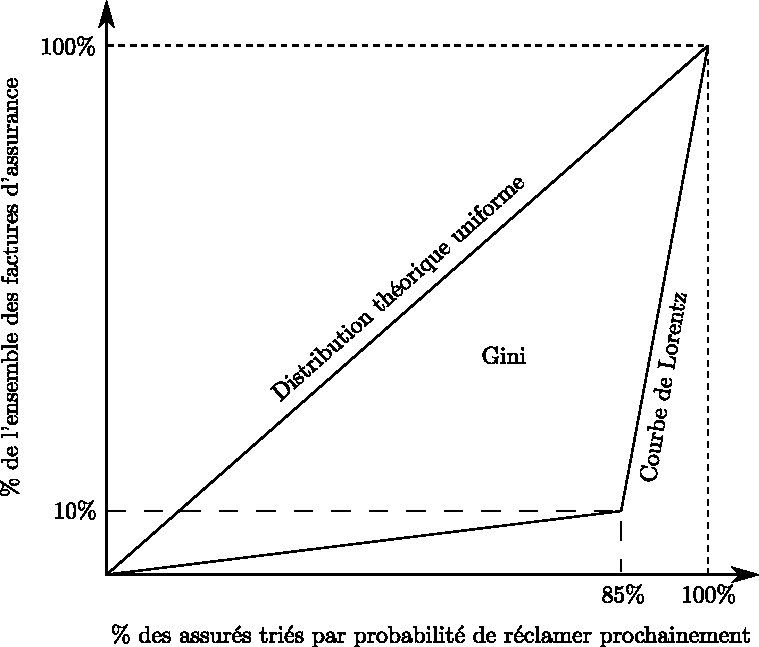
\includegraphics[width = \columnwidth]{img/gini}
%  \caption{Coefficient de Gini et Courbe de Lorentz}
%\end{figure}


%Une lecture de la courbe de Lorentz (figure 1) serait \og les 15\% des assurés les plus risqués paient 90\% de l'ensemble des factures d'assurance \fg{}. Ceci correspond bien au principe de mutualisation des risques qui correspond à la base des systèmes d'assurance. Ainsi, plus le coefficient de Gini est élevé, plus la capacité à individualiser les tarifs sera bonne. La normalisation de ce coefficient permet de s'assurer que la valeur prise par la métrique va de 0 (aucune capacité prédictive) à 1 (capacité prédictive parfaite).

\subsection{Benchmark d'ouverture}

Il est intéressant de placer un benchmark afin d'avoir une valeur de la métrique objectif (Coefficient Normalisé de Gini) à dépasser. Le score obtenu par un Light GBM\footnote{Gradient Boosting Machine} est généralement élevé et rapidement obtenu. Celui-ci est de : 0.2719 par validation croisée sur 5 blocs (5fCV). La réalisation d'un score obtenu par la méthode du Light GBM est effectuée à chaque étape du traitement : sélection de variables, regroupement par classe, normalisation des données, paramétrisation des modèles. La variation de ce score lors des ces différentes étapes permettra d'évaluer leur pertinence. 


\subsection{Pré-traitement des données}

Le pré-traitement des données consiste essentiellement à la gestion des valeurs manquantes. Plusieurs variables ont été identifiées dans les statistiques descriptives (\emph{Figure 1}). Selon le taux de valeurs absentes, la manipulation appliquée sera différente. 

\begin{figure}[H] \centering
  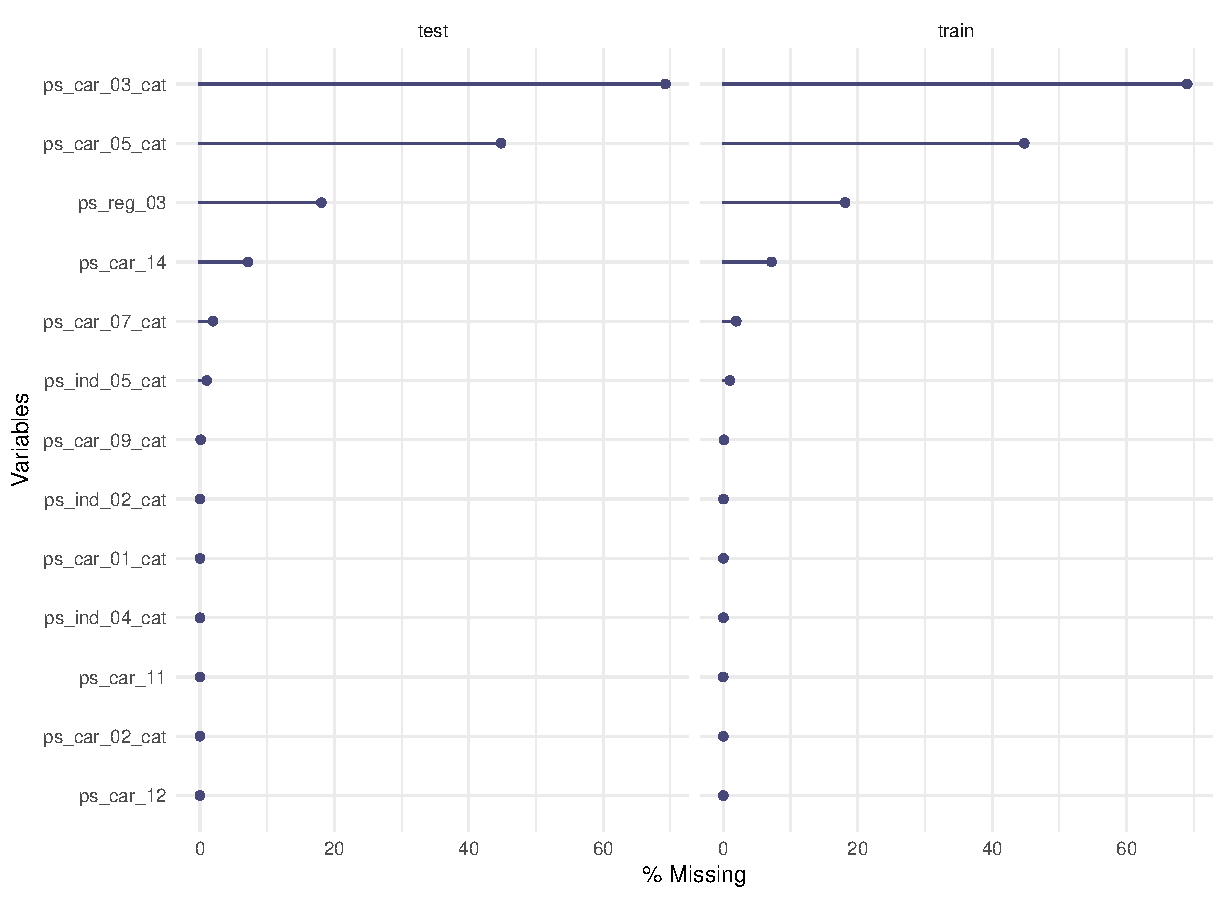
\includegraphics[width = \columnwidth]{img/missing_values}
  \caption{Valeurs manquantes par variable}
\end{figure}

Deux variables explicatives  qualitatives présentent trop de valeurs manquantes (plus de 40\%) ce qui pourrait conduire à supprimer ces variables de l'étude. Cependant, la comparaison de ces variables avec la cible montre que la perte de ces valeurs manquantes serait une perte d'information. Le nombre élevé de valeurs manquantes ne permet pas une imputation sophistiquée pour ces variables. Les valeurs manquantes de ces deux variables qualitatives sont remplacées par une valeur spéciale (-999 par exemple), permettant ainsi de conserver l'information issue de l'absence de valeur.

Pour le reste des variables, une imputation par forêt aléatoire est faite. Le procédé d'imputation est le suivant :
\begin{itemize}
    \item Utiliser uniquement l'échantillon d'apprentissage pour construire la forêt aléatoire.
    \item Modéliser la variable étudiée en s'assurant qu'il s'agisse du bon type d'arbres (classification ou régression) en utilisant les autres variables comme régresseurs.
    \item Prédire les valeurs de la variable étudiée pour l'ensemble des observations manquantes des deux échantillons (apprentissage et test).
    \item Remplacer les valeurs manquantes et s'assurer qu'il n'y a plus de valeurs manquantes pour la colonne traitée.
\end{itemize}

Suite aux imputations faites, le Light GBM de référence renvoie un score de Gini de 0.2721, toujours par validation croisée sur 5 blocs. On note une augmentation par rapport au benchmark bien que la différence soit trop faible pour en tirer des conclusions.

\subsection{Sélection des variables}

Le Light GBM effectué après les imputations permet également d'identifier l'importance des variables dans le pouvoir prédictif du modèle. L'importance d'une variable peut être mesurée de différentes manières. Celle adoptée ici est le \og Gain \fg \cite{twds1}, i.e. la contribution de la variable au modèle.  Cette contribution se décompose comme étant la variation de la fonction d'impureté entre les deux nouveaux nœuds et le nœud initial. Un terme de régularisation intervient dans le calcul et si celui-ci est supérieur en valeur absolu à la variation de la fonction d'impureté, alors il n'y a pas d'intérêt à effectuer le split en question \cite{wittkowski1986classification}.


Ainsi, plus une variable contribue au pouvoir prédictif d'un modèle, plus son \og Gain \fg{} associé sera élevé. Arbitrairement, on garde la première moitié des variables les plus contributives au modèle.

\begin{figure}[H] \centering
  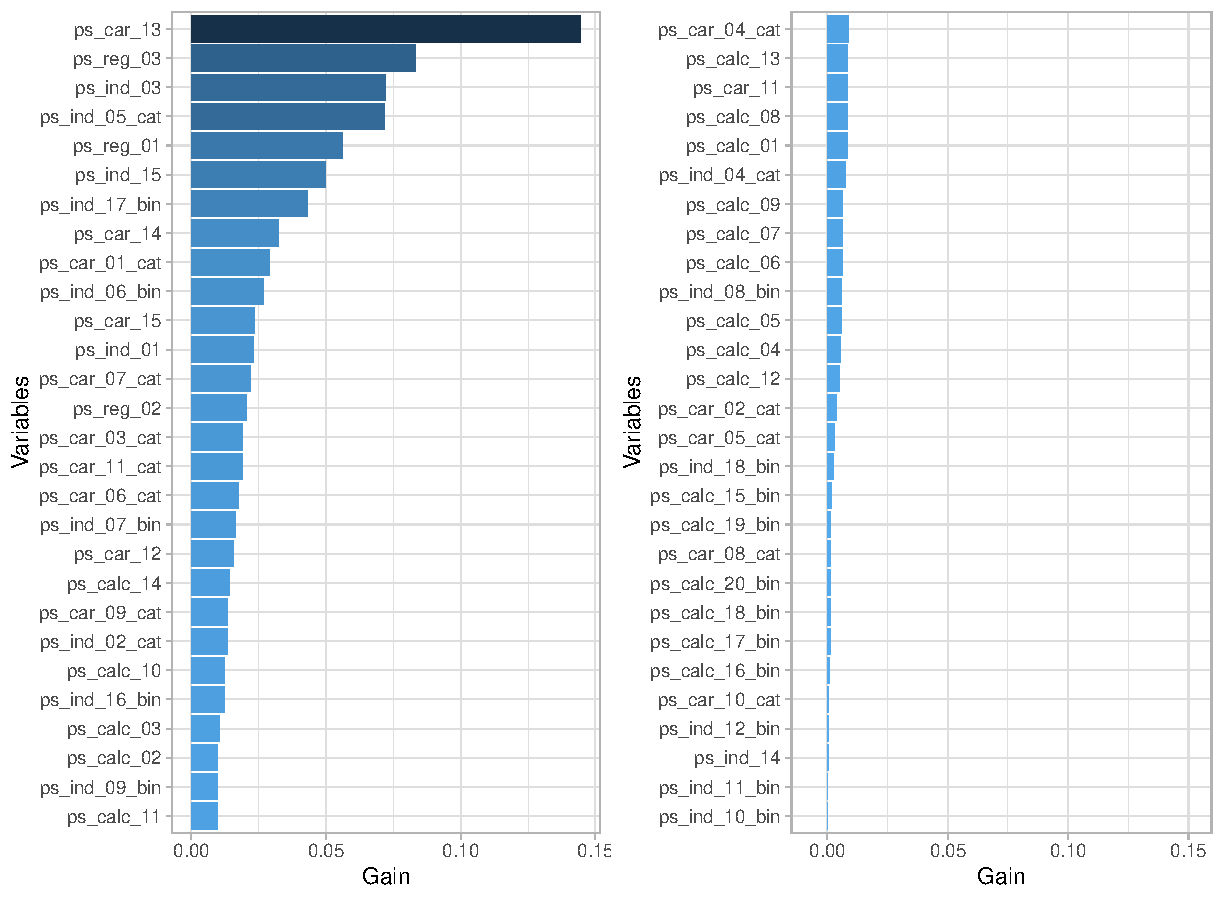
\includegraphics[width = \columnwidth]{img/var_imp_lgb}
  \caption{Importance des variables}
\end{figure}

En plus des importances issues du LightGBM, une forêt aléatoire (sans optimisation des hyper-paramètres) est construite pour réaliser une seconde liste d'importance en termes de \og Permutation \fg{} \cite{rb1}. Ainsi, une seconde liste de variables est identifiée en sélectionnant la moitié des variables les plus importantes au modèle au sens de la notion de \og Permutation \fg. L'union de ces deux listes constitue la liste finale des variables retenues pour la suite. Cette liste mélange des variables importantes selon la fonction d'impureté choisie (gain) et/ou le taux de bonnes réponses (permutation). Au total, ce sont 35 régresseurs sur les 57 initiaux qui sont retenus.

\subsection{Traitement des données}

Plusieurs variables présentent des modalités rares (effectif inférieur à 5\%). Il est difficile d'obtenir des résultats d'estimation robustes pour ces modalités. Il est donc nécessaire de fusionner certaines modalités. Cependant, les modalités de ces variables ont été anonymisées, il n'est donc pas possible de les regrouper par l'intermédiaire d'une certaine expertise. Dans le but de fusionner ces modalités rares, deux stratégies ont été testées :  l'Analyse Factorielle de Données Mixtes (AFDM) et les tableaux de contingence.

La stratégie de fusion peut passer par une projection des modalités d'une variable sur le premier plan factoriel d'une AFDM. Chaque modalité rare sera alors associée à la modalité fréquente la plus proche d'elle (et si possible projetée dans la même direction), ou un ensemble de modalités rares peuvent se regrouper pour former un groupe supplémentaire (clusters).

La stratégie de fusion peut également passer par des tableaux de contingence (\emph{Figure 3}) qui croisent les variables avec la cible. Les modalités rares sont fusionnées soit entre elles si elles se comportent de façon similaire, soit avec une modalité fréquente si le comportement s'en rapproche.

\begin{figure}[H] \centering
  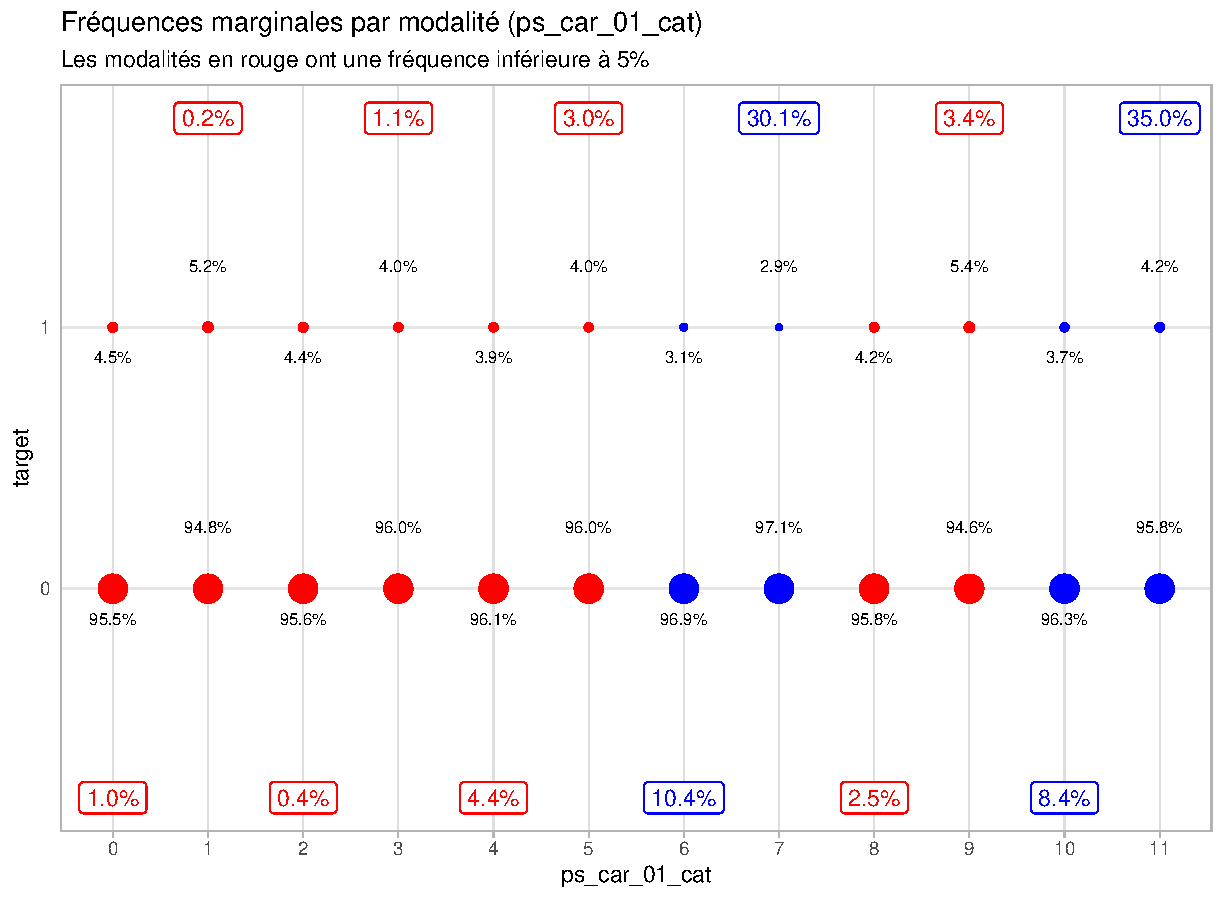
\includegraphics[width = \columnwidth]{img/ex_tabc}
  \caption{Exemple de projection de modalités par croisement}
\end{figure}

Une variable présente un grand nombre de modalités (104). Plutôt que de fusionner ces modalités, on peut s'en servir comme régresseur unique d'une régression logistique avec la variable cible comme variable à expliquer. Les modalités seront alors remplacées par les coefficients estimés et la variable deviendra alors numérique et continue.

Le Light GBM fournit un score de 0.2729 (5fCV) pour la stratégie par AFDM et de 0.2757 (5fCV) pour la stratégie par tableaux croisés. Ces deux scores sont supérieurs à celui du benchmark. Cependant, nous retiendrons la deuxième stratégie car elle permet l'obtention d'un meilleur score par rapport à la première.

\subsubsection{Normalisation des données}

Certaines variables continues ont une distribution qui ont un fort kurtosis (i.e. avec un haut sommet) et qui n'est pas centrée. Il serait donc intéressant de tenter de les transformer à travers différentes méthodes (box-cox, logarithme, racine carré).

\begin{figure}[H] \centering
  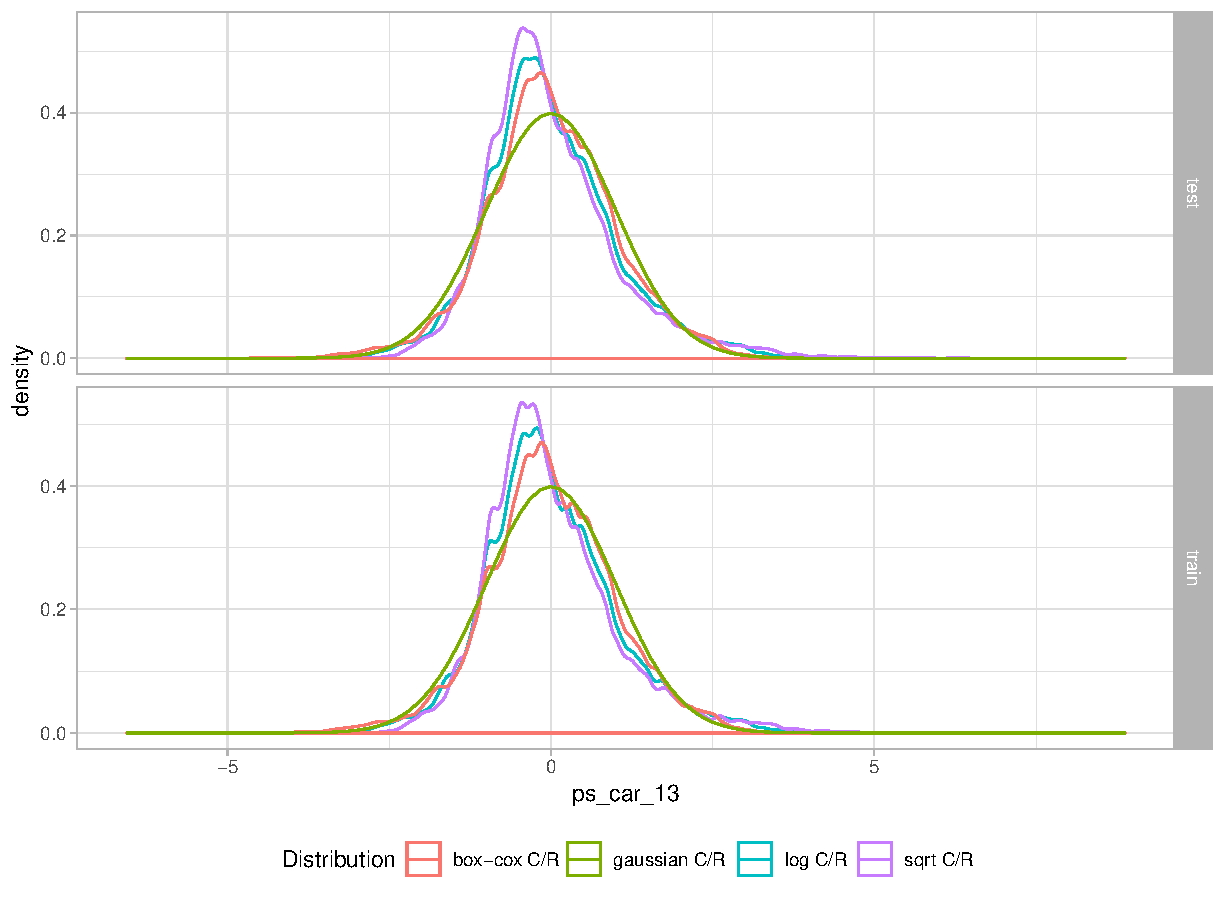
\includegraphics[width = 0.99\columnwidth]{img/ex_normalisation}
  \caption{Exemple de transformation}
\end{figure}

Il est notable que la transformation de box-cox est la meilleure pour normaliser cette distribution (\emph{Figure 4}). Cette étude est menée pour les variables continues.

En réutilisant un Light GBM pour mesurer les conséquences des transformations réalisées, il est noté que la métrique diminue, suite à chacune des deux stratégies de fusion de modalités. On passe respectivement à un score de Gini de 0.2729 pour l'AFDM et de 0.2752 pour les tableaux croisés. Ces diminutions sont minimes mais la transformation des variables n'est pas obligatoire. Par conséquent, cette étape est laissée de côté pour la suite. 

À la fin de cette étape, le traitement se résume à la fusion de modalités en utilisant des tableaux de contingence.

\subsection{Étude des corrélations et dépendances}

L'objectif de cette étape est d'étudier les liens entre variables. On évalue les corrélations et les dépendances entre variables puis avec la cible. Ceci permet de détecter des problèmes de colinéarité et ou dépendance entre prédicteurs :

\begin{itemize}
    \item les liens entre variables continues se font grâce aux corrélations,
    \item les liens entre les variables continues et la cible se font grâce à un test d'ANOVA\footnote{Analysis of Variance},
    \item les liens entre variables catégorielles (et la cible) se font grâce aux V de Cramer\footnote{Le V de Cramer est la statistique du $\chi^2$ standardisée de façon à ce qu'elle varie entre 0 et 1}.
\end{itemize}

Les variables qui dépassent les seuils arbitrairement fixés ou qui ne passent pas le test d'ANOVA sont laissées de côté. L'étude n'a pas abouti à de suppression de variables.

\subsection{Paramétrisation des modèles}

Une dizaine d'algorithmes sont construits afin de s'approcher du meilleur pouvoir prédictif tels que : l'Analyse Discriminante Linéaire (LDA), les K plus proches voisins (KNN), la régression logistique (pénalisée ou non), la Machine à Vecteurs de Support (SVM)), puis des modèles de bagging (Forêt Aléatoire) et de boosting (ADAboost, GBM, XGBM, LGBM).

L'ensemble des modèles ensemblistes et la régression logistique pénalisée sont optimisés selon leurs hyper-paramètres\footnote{Les algorithmes KNN et SVM ne sont pas optimisés faute du temps d'exécution nécessaire au calcul de matrices immenses de distance}. La méthode choisie pour effectuer cette hyper-paramétrisation est celle du \og grid search\fg. L'idée étant d'établir au préalable une liste arbitraire non exhaustive de valeurs des hyper-paramètres puis de retenir la combinaison qui maximise le score de Gini pour chaque modèle. 

Le fait que les données soient déséquilibrées pose la question du ré-échantillonnage. Ainsi, pour l'ensemble des modèles, les stratégies de down-sampling, up-sampling et SMOTE sont testées en plus du jeu de données d'apprentissage initial. L'hyper-paramétrisation via la méthode du \og grid search \fg   \ est donc effectuée pour ces quatre cas.



\section{Méthodes utilisées}
L'intuition et le fonctionnement de trois méthodes sont détaillés dans cette section. La régression logistique pénalisée sera présentée en premier, suivie de deux méthodes de boosting : le XGboost et le LightGBM. La régression logistique pénalisée a des principes radicalement différents des deux méthodes de boosting.


\subsection{Régression logistique pénalisée}
La pénalisation de la métrique optimisée pour estimer les paramètres est un principe applicable à toutes les méthodes d'estimation où l’on a des combinaisons de variables avec des coefficients à estimer (réseaux de neurones, SVM linéaire, etc).\\
L'idée étant que les hypothèses classiques de la régression linéaire permettent d'obtenir le meilleur estimateur non biaisé i.e. l'estimateur sans biais de variance minimale. Dans les faits on obtient un estimateur de faible biais mais de variance plus élevée car ces hypothèses ne sont jamais totalement respectées.

Or, en considérant l'écart quadratique moyen (EQM) qui est la fonction de perte la plus largement utilisée on a : 
\[\mathbb{E}\left[\left(y^{*}-\hat{y}^{*}\right)^{2}\right]=\sigma^{2}+\left(\mathbb{E}\left[\hat{y}^{*}\right]-y^{*}\right)^{2}+\mathbb{E}\left[\left(\hat{y}^{*}-\mathbb{E}\left[\hat{y}^{*}\right]\right)^{2}\right] \]

On a respectivement $\sigma^{2}$ la variance incompressible de la cible Y, le biais au carré et la variance de la prévision. Ainsi si on s'autorise un certain biais, on peut imaginer qu'il est possible de réduire plus que proportionnellement la variance et ainsi gagner en pouvoir prédictif.
En pratique, on cherche le meilleur compromis entre le biais et la variance.\\
Dans le cadre classique de la discrimination binaire par la régression logistique, on suppose $(x_i,y_i)$ \emph{iid} d'une même distribution inconnue.\\
On modélise $\mathbb{P}(Y=1|X=x_i)=\frac{1}{1+e^{-\left(\beta^{\prime} x\right)}}=p_i$.

\noindent Une approche \cite{art3} consiste à résoudre le problème suivant : 
\[ \left| \begin{array}{l}\displaystyle\min_{\beta}-\frac{1}{n} \sum_{i=1}^{n} \left[y_{i} \ln p_{i}+\left(1-y_{i}\right) \ln \left(1-p_{i}\right)\right] + R(\beta) \\
\text{sous contraintes : } R (\beta) \leq \tau \end{array} \right.\]
qui s'écrit également : 
\[\ \displaystyle\min_{\beta}-\frac{1}{n} \sum_{i=1}^{n} \left[y_{i} \ln p_{i}+\left(1-y_{i}\right) \ln \left(1-p_{i}\right)\right] +\lambda R(\beta) \]\
où l'on aura pris soin de centrer et réduire les variables afin de leur accorder la même importance.
\\

\noindent Il y a 3 types de pénalisation utilisés régulièrement: 
\begin{enumerate}
    \item en norme $L^{2}$ on parle alors de régression ridge  : \ $R(\beta)=\sum_{j=1}^{p}\beta_{j}^{2}$
    \item en norme $L^{1}$ on parle alors de régression LASSO  : $R(\beta)=\sum_{j=1}^{p}\left|\beta_{j}\right|$
    \item ElasticNet qui est une combinaison linéaire des 2 : $R(\beta)=\alpha \sum_{j=1}^{p}\left|\beta_{j}\right|+(1-\alpha) \sum_{j=1}^{p} \beta_{j}^{2}$
\end{enumerate}

À noter que $\lambda$ est un paramètre du modèle qu'il faut calibrer également.\\
On a une relation inverse entre $\tau$ et $\lambda$. Lorsque $\lambda=0$ on retrouve les MCO et plus $\lambda$ est grand, plus les coefficients sont contraints (plus de biais, moins de variance).
On peut voir les coefficients se déformer en fonction de $\lambda$.\\
La régularisation dans la régression ridge est plus souple que dans la régression LASSO qui force les coefficients des variables moins explicatives à 0.\\ Il peut s'agir d'une procédure de sélection de variables.
Un des inconvénients de la régression LASSO est qu'elle choisit arbitrairement une variable parmi un groupe de variables corrélées tandis que la régression ridge permet de pondérer les influences.\\
L'Elastic Net permet de combiner les avantages des deux méthodes en contrepartie d'une complexité accrue.\\

Pour choisir $\lambda$, on procède généralement par apprentissage-test lorsque c'est possible ou par validation croisée K-folds lorsque la base est petite, en minimisant un critère d'erreur. Des formules basées sur des hypothèses simplificatrices existent également.\\

\noindent Pour la régression ridge, à $\lambda$ donné on a : $$ \hat{\beta}_{\lambda}^{\text {ridge}}=\left(\mathrm{X}^{\prime} \mathrm{X}+\lambda l_{p}\right)^{-1} \mathrm{X}^{\prime} Y$$
Pour la régression LASSO (sachant que la fonction $\beta \mapsto\|Y-\mathbb{X} \beta\|_{2}^{2}+\lambda\|\beta\|_{1}$ est convexe mais non différentiable), le minimum global de la fonction objectif existe mais il n'y a pas de stricte convexité, ce qui entraîne la non unicité de la solution optimale $\beta_{\lambda}$.
On obtient $\beta_{\lambda}$ par optimisation de la fonction objectif par descente de coordonnées (package glmnet sous R).\\
L'idée est d'optimiser chaque $\beta_j$ un à un \cite{fromont} (on considère les autres coefficients comme constants dans la fonction objectif) en effectuant un certain nombre d'itérations ou jusqu'à obtenir une variation de $\beta$ suffisamment faible ($ <\epsilon $ fixé).

\subsection{Gradient Boosting Machine}
\subsubsection{XGboost}
L’algorithme XGboost est l'abréviation de e\textbf{X}treme \textbf{G}radient \textbf{boost}ing, approche introduite par Friedman\footnotemark[11].\\
Comme la plupart des méthodes basées sur des arbres de décisions, il peut être utilisé en classication comme en régression.\\
L'approche combine 2 mécanismes : le boosting et la descente de gradient.\\
Le boosting est une méthode ensembliste qui consiste à agréger des classifieurs élaborés séquentiellement sur un échantillon d’apprentissage dont les poids des individus sont corrigés au fur et à mesure, les individus mal classés se voyant affecter un poids plus important. Les classifieurs sont pondérés selon leurs performances.\\
D'autre part, la descente du gradient est une technique itérative qui permet d’approcher la solution d’un problème d’optimisation \cite{art1}.\\
Enfin, outre les deux mécanismes précédents, l’approche possède aussi des paramètres liés à l’utilisation d’arbres comme classifieurs.\\
Ainsi, l’algorithme XGboost dépend d’un grand nombre d' hyperparamètres: 
\begin{enumerate}
    \item Caractéristiques des
arbres individuels : Profondeur T, effectifs minimums de coupe 
\item Constante
d'apprentissage $\eta$
\item Nombre d'arbres K
\item Taux d'échantillonnage des individus $\beta$
\item Échantillonnage des variables
\end{enumerate}
On optimise les hyperparamètres par grid search.\\
L'algorithme propose également une gestion efficace de matrices creuses et des valeurs manquantes : \og sparsity-aware split finding \cite{chen2016xgboost} \fg{}. Ces valeurs manquantes sont dirigées vers le noeud qui optimise le gain.

La prévision se base sur K arbres construits de façon itérative. À chaque étape on ajoute celui qui minimise une fonction objectif régularisée $\mathcal{L}$ qui est la somme d'une fonction de perte et d'une fonction de régularisation\footnotemark[11].\\
\[\ \mathcal{L}=\sum_{i} l\left(\hat{y}_{i}, y_{i}\right)+\sum_{k} \Omega\left(f_{k}\right) \]\\
$\text {avec } \Omega(f)=\gamma T+\frac{1}{2} \lambda\|w\|^{2}$, $\gamma$ étant le coefficient de pénalisation par rapport à la profondeur $T$, $\lambda$ le coefficient par rapport qui pondère l'impact du poids $w$.
\\
La fonction de perte est généralement la déviance binomiale en classification binaire :\\
 \[\ -\frac{1}{n} \sum_{i=1}^{n} \left[y_{i} \ln p_{i}+\left(1-y_{i}\right) \ln \left(1-p_{i}\right)\right] \]
On utilise la descente de gradient pour optimiser cet objectif à chaque étape.\\
L'optimisation est effectuée sans les valeurs manquantes pour le feature considéré, les individus ayant le feature manquant pour le noeud optimal sont affectés à la direction majoritaire.\\
L'algorithme réalise un one-hot encoding\footnote{consistant à construire autant de variables binaires que de valeurs possibles prises par la variable catégorielle (binarisation)} des variables catégorielles pour pouvoir calculer le gain.\\
Pour accélérer l'optimisation, une approximation d'ordre 2 de la fonction objectif est faite\footnotemark[11].\\
\[\ \mathcal{L}^{(t)} \simeq \sum_{i=1}^{n}\left[l\left(y_{i}, \hat{y}^{(t-1)}\right)+g_{i} f_{t}\left(\mathbf{x}_{i}\right)+\frac{1}{2} h_{i} f_{t}^{2}\left(\mathbf{x}_{i}\right)\right]+\Omega\left(f_{t}\right) \]\ 
avec  
\[ g_{i}=\partial_{\hat{y}(t-1)} l\left(y_{i}, \hat{y}^{(t-1)}\right) \ \text{ et } \ h_{i}=\partial_{\hat{y}(t-1)}^{2} l\left(y_{i}, \hat{y}^{(t-1)}\right)\]
Considérer l'ensemble des noeuds possibles est impossible, une heuristique gloutone\footnote{algorithme qui visite itérativement son voisinage pour optimiser l'objectif} basée sur un ensemble de noeuds éligibles est couramment utilisée.\\
L'algorithme XGboost est dit \og Leaf-wise \fg{}, il est construit en profondeur.\\
On peut determiner le poids optimal de chaque noeud en différenciant la fonction objectif que l'on utilise également comme une mesure d'impureté.\\
%$$
%\mathcal{L}_{\text {split}}=\frac{1}{2}\left[\frac{\left(\sum_{i \in I_{L}} g_{i}\right)^{2}}{\sum_{i \in I_{L}} h_{i}+\lambda}+\frac{\left(\sum_{i \in I_{R}} g_{i}\right)^{2}}{\sum_{i \in I_{R}} h_{i}+\lambda}-\frac{\left(\sum_{i \in I} g_{i}\right)^{2}}{\sum_{i \in I} h_{i}+\lambda}\right]-\gamma
%$$
$$
\mathcal{L}_{\text {split}}=\frac{1}{2}\left[\frac{\displaystyle\left(\sum_{i \in I_{L}} g_{i}\right)^{2}}{\displaystyle\sum_{i \in I_{L}} h_{i}+\lambda}+\frac{\displaystyle\left(\sum_{i \in I_{R}} g_{i}\right)^{2}}{\displaystyle\sum_{i \in I_{R}} h_{i}+\lambda}-\frac{\displaystyle\left(\sum_{i \in I} g_{i}\right)^{2}}{\displaystyle\sum_{i \in I} h_{i}+\lambda}\right]-\gamma
$$
où $I_{R}$ et $I_{L}$ sont les noeuds droit et gauche issus du noeud $I$.\\
Une optimisation de l'algorithme d'évaluation des coupes basée sur les quantiles et le nombre de noeuds voulus pour chaque feature (basé sur un scoring via les gradiants de premier ordre) est utilisée en grande dimension.\\
On peut ajouter de l'aléa dans l'échantillon test en utilisant seulement un échantillon des données pour construire les arbres. Ceci a l'avantage d'accélérer les calculs et de se prémunir contre le surapprentissage.\\
Il est évident que plus le nombre d'itérations est grand, plus on s'approche de la solution optimale, cependant celà s'effectue au détriment du temps de calcul.\\
Le compromis pour $\eta$ $\in$ $]0,1[ $ est réalisé entre vitesse de convergence et surapprentissage.\\
Si l'algorithme est très efficace, souple avec le choix des fonctions de coûts,
adaptables à différents problèmes, permettant de prendre efficacement en compte des interactions non linéaires, cela conduit à une procédure difficilement interprétable (bien qu'on puisse calculer des mesures d'importance des variables), lourde en mémoire et intensive avec beaucoup de paramètres à optimiser et un risque de surapprentissage qui peuvent rendre sa mise en œuvre moins aisée.

\subsubsection{LightGBM}
L'algorithme LightGBM est une autre implématation du Gradient Boosting Tree, très efficace en mémoire et en temps de calcul.\\
Il s'agit également d'un algorithme \og Leaf-wise \fg{}.\\
Les deux principales différences avec XGboost sont des approches heuristiques pour diminuer drastiquement le temps de calcul tout en restant très performant.\\
Une première approche pour reduire le nombre d'observations à prendre en compte pour calculer le split est appelée GOSS : \og Gradient-based One-Side Sampling \fg{} \cite{micr}.\\
L'idée étant que les observations avec un faible gradient sont peu informatives, les a\% premières observations triées par gradient decroissants sont conservées (ensemble $A$) puis on prend aléatoirement b\% du reste (ensemble $B$).\\
Afin de ne pas trop modifier la distribution des observations, on multiplie les gradients des observations échantillonnées par un facteur $\frac{1-a}{b}$ dans la mesure de gain de variance $\tilde{V}_{j}$.\\
\[
\tilde{V}_{j}(d)=\frac{1}{n}\left(\frac{\left(\sum_{x_{i} \in A_{l}} g_{i}+\frac{1-a}{b} \sum_{x_{i} \in B_{l}} g_{i}\right)^{2}}{n_{l}^{j}(d)} \right. \]
\[ \null \qquad \qquad + \left. \frac{\left(\sum_{x_{i} \in A_{r}} g_{i}+\frac{1-a}{b} \sum_{x_{i} \in B_{r}} g_{i}\right)^{2}}{n_{r}^{j}(d)}\right)
\]
avec $A_l$ et $B_l$ correspondant au subset des parties $A$ et $B$ au point de coupure $d$ pour le feature $j$ dans la feuille gauche, de même pour $A_r$ et $B_r$ pour le côté droit; $n_l^j$ et $n_r^j$ sont les nombres d'observations respectifs\footnotemark[14].

Une borne supérieure de l'erreur commise est connue théoriquement, on peut déduire de celle-ci que si le nombre d'observations est grand et que le seuil selectionné n'induit pas un déséquilibre des observations important alors l'approximation est excellente.\\
L'erreur de généralisation via GOSS (comparaison avec le gain de variance sur toutes les données (\og vraie variance de la distribution \fg{})) est très bonne si l'erreur du GOSS est déja bonne sinon un sampling classique des observations peut permettre de mieux apprendre.\\
On comprend pourquoi on n'a pas intérêt à échantillonner le training set pour cet algorithme, ce qui transparait bien dans nos résultats.

La deuxième approche est appélée Exclusive Feature Bundling (EFB)\footnotemark[14].\\
Le but est d'aggréger intelligement les variables qui ne sont pas ou peu mutuellement nulles simultanement.\\
Il s'agit d'un problème NP-difficile donc une heurtistique gloutone est utilisée.\\
On aggrège les variables de manière itérative dans des \og bundles \fg{} jusqu'à obtenir un seuil de conflit prédéfini.\\
On parvient à diminuer drastiquement le nombre de features.\\
C'est la réduction à la fois du nombre d'observations et du nombres de features à scanner qui rend cet algorithme si rapide. Cette approche est plus efficace que le Stochastic Gradient Boosting.







\section{Résultats}

L'approche GOSS du LightGBM explicitée dans la section précédente incite à ne pas effectuer de reéchantillonnage. La valeur dans la colonne \og up \fg{} (0.2762) est obtenue en pondérant le poids des \og 1 \fg{} par 26 contre 1 en réalité (\emph{Table 1}).

\captionof{table}{Coefficient normalisé de Gini en validation croisée}
\begin{center}\begin{tabular}{|l|r|r|r|r|} \hline
  & \multicolumn{1}{c|}{down} & \multicolumn{1}{c|}{up} & \multicolumn{1}{c|}{SMOTE} & \multicolumn{1}{c|}{aucun} \\ \hline
  ElasticNet & 0.2566 & 0.2576 & 0.2483 & 0.2573 \\
  XGboost & 0.2678 & 0.2728 & 0.2687 & 0.2778 \\
  LightGBM & . & 0.2762 & . & 0.2757 \\ \hline

\end{tabular}\end{center}



La régression logistique pénalisée présente des performances inférieures aux deux méthodes de boosting. Ceci peut s'expliquer par son incapacité à expliquer des phénomènes non-linéaires. Les méthodes de boosting apprennent séquentiellement de leurs erreurs et deviennent rapidement des boîtes noires à pouvoir prédictif élevé.

\subsection{Comparaison avec d'autres algorithmes}

Plusieurs autres modèles ont été paramétrés par \og grid search \fg{} pour chaque stratégie de resampling puis évalués en validation croisée 5 blocs. La \emph{Figure 5} répertorie les résultats de performance obtenus.

\begin{figure}[H] \centering
  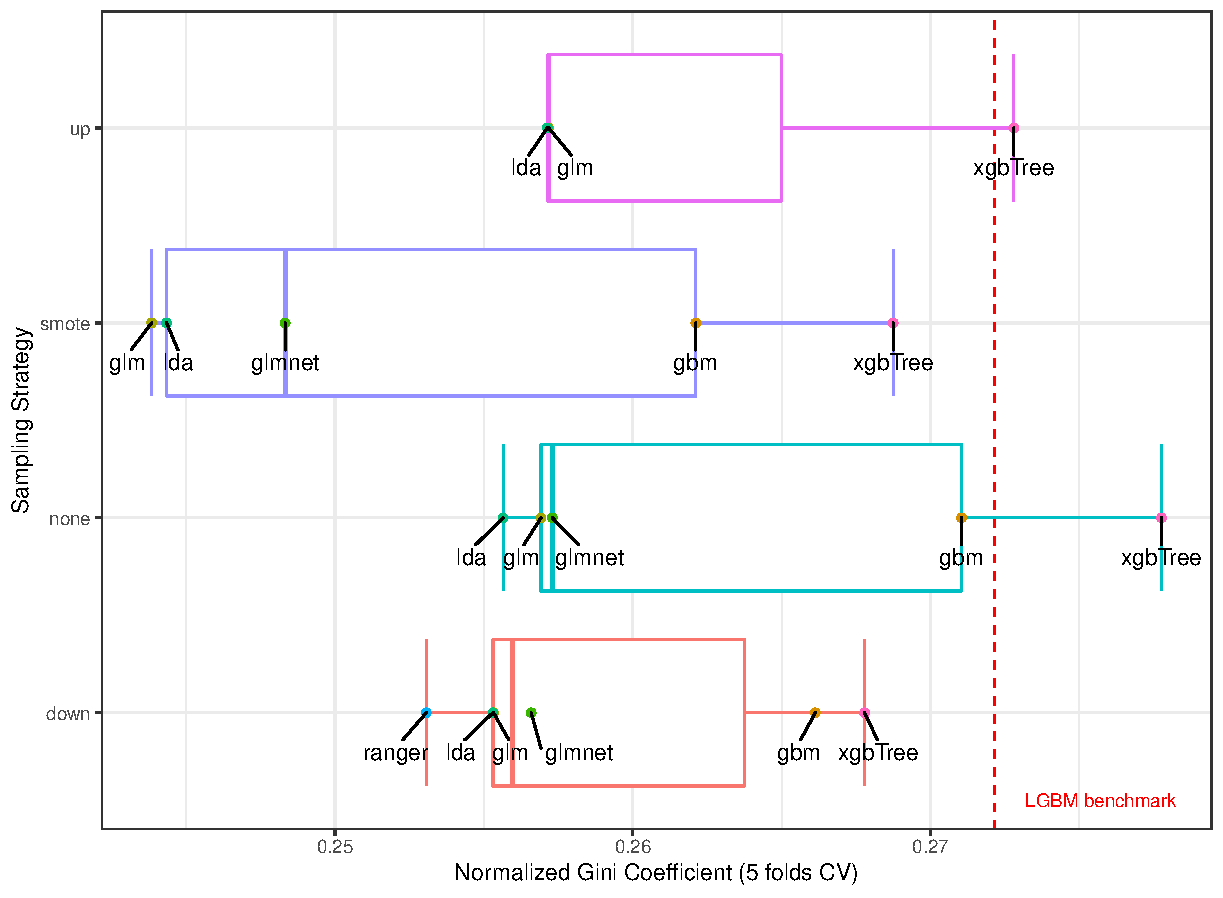
\includegraphics[width = \columnwidth]{img/results}
  \caption{Performance de validation des modèles}
\end{figure}

Certains modèles construits tels que les arbres de décision ne figurent pas dans la figure parce que leur performance est trop faible. Les modèles de stacking (\emph{glm\_stack} et \emph{combi}) ont été construits en choisissant les deux modèles les plus performants. Le méta-classifieur du stacking est une régression logistique et le modèle \og combi \fg{} correspond à un classifieur qui combine linéairement les scores issus de la validation croisée des modèles. Pour les deux modèles de stacking, seules les prédictions issues du Light GBM et du XGboost (sans reéchantillonnage) sont utilisées.

Bien que les performances des modèles ayant appris sur des données sur-échantillonnées sont équivalentes à celles des modèles sans reéchantillonnage, deux raisons vont en faveur de la seconde solution :
\begin{itemize}
    \item le sur-échantillonnage engendre une augmentation des temps de calcul (duplication des individus, apprentissage sur quasiment deux fois plus de données)
    \item le meilleur modèle en validation croisée est obtenu sans reéchantillonnage.
\end{itemize}
Par conséquent, seuls les modèles sans reéchantillonnage seront retenus afin de tracer leur courbe ROC (\emph{Figure 6}).

\begin{figure}[H] \centering
  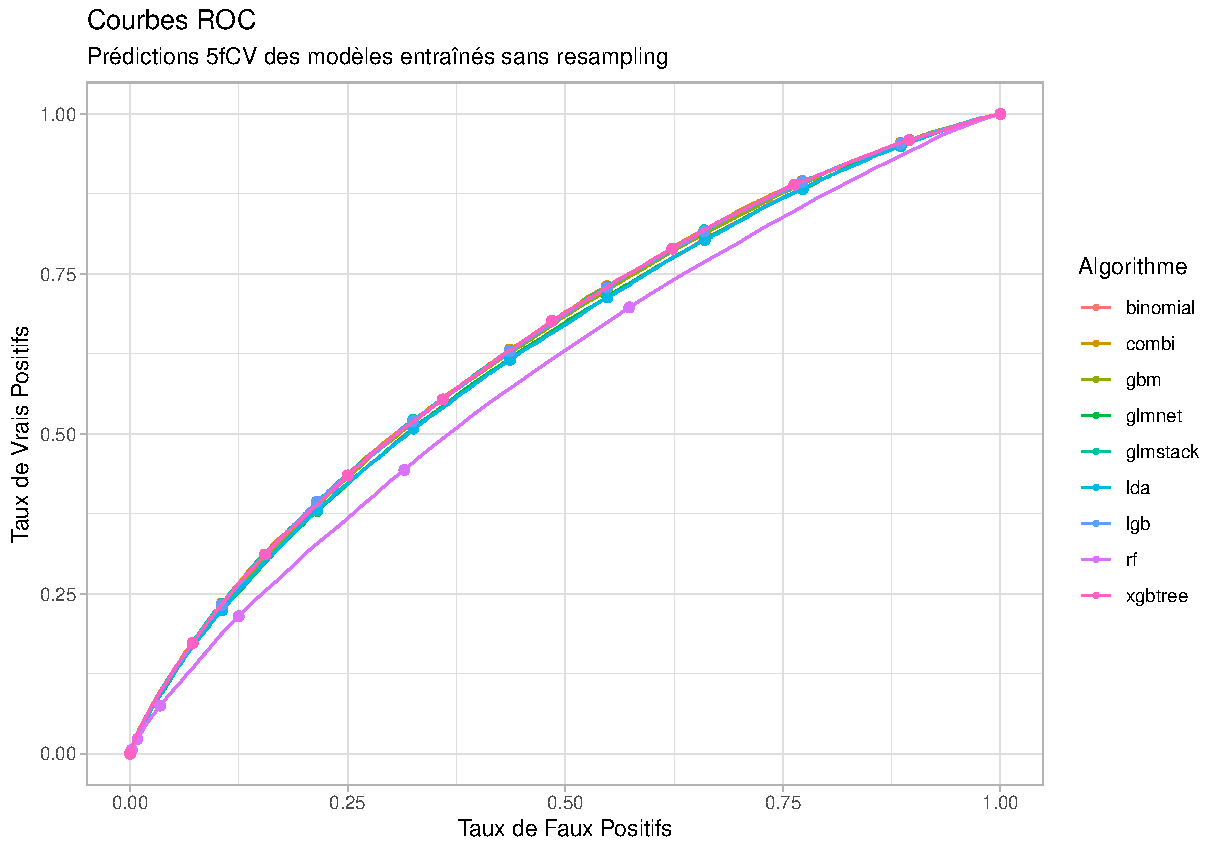
\includegraphics[width = \columnwidth]{img/roc_curves}
  \caption{Courbes ROC des modèles sans reéchantillonnage}
\end{figure}

Finalement, le modèle combiné dépasse le reste des modèles avec un coefficient normalisé de Gini en validation croisée de 0.2794. L'application à l'échantillon test renvoie une valeur de 0.2881\footnote{À titre informatif, l'AUROC (Area Under the Receiver Operating Characteristic curve) du modèle sur l'échantillon test est de 0.6440.}.

\

Pour passer de la prédiction à la classification \cite{fhar}, il est nécessaire de fixer un seuil pour lequel les scores en-dessous de celui-ci correspondent à un label \og 0  \fg{} pour les individus concernés et \og 1 \fg{} sinon. L'obtention de ce seuil dépend de l'objectif à maximiser (le score F1 semble être le plus approprié dans ce contexte (données déséquilibrées)) et doit se faire sur les prédictions issues de la validation croisée. Le seuil retenu est ensuite utilisé sur l'échantillon test afin de vérifier la stabilité entre la validation et le test.
\columnbreak

Les résultats suivants sont obtenus :

\captionof{table}{Performances de classification pour un seuil défini}
\begin{center}\begin{tabular}{|l|r|r|} \hline
  & F1 & Rappel \\ \hline
  Échantillon de Validation & 0.1176 & 0.2482 \\
  Échantillon Test & 0.1158 & 0.2488 \\ \hline
\end{tabular}\end{center}

Le F1 (ou score F1) dépend à la fois du Rappel\footnote{taux de vrais positifs sur l'ensemble des vrais observés} et de la Précision\footnote{taux de vrais positifs sur l'ensemble des vrais prédits} des prédictions et est une métrique adaptée en situation de déséquilibre de la variable cible. Dans le contexte d'une assurance, le Rappel est plus important que la Précision car une faible valeur du Rappel indiquerait que la tarification appliquée est trop faible par rapport au risque du client. Ici, un client sur quatre labélisé \og 1 \fg{} en réalité est détecté par l'algorithme (\emph{Tables 2 et 3}). Pour aller plus loin, la connaissance métier permettrait d'affiner le score F1 en pondérant correctement la Précision et le Rappel.

%\begin{multicols}{2}


\captionof{table}{Matrice de confusion (échantillon test)}
{\footnotesize{\begin{center} \begin{tabular}{|cc|c|c|} \hline
  & & \multicolumn{2}{c|}{Observé} \\
  & & 0 & 1 \\ \hline
  \multirow{2}{*}{\rotatebox{90}{Prédiction \ }} & 0 & 152 542 & 4 827 \\[15pt] \cline{2-4}
  & 1 & 19 596 & 1 599 \\[15pt] \hline \end{tabular} \end{center}}}
  
  Le passage d'un score à un label reste au choix d'arbitrage du décideur (assureur), basé sur les enseignements tirés de cette matrice de confusion mais également d'autres éléments non étudiés ici : interprétation et explicativité des variables (méthode LIME\cite{ribeiro2016should} ou méthode Shapley\cite{vstrumbelj2014explaining}).

\end{multicols}

%\vfill\null
%\noindent \vhrulefill{1.5pt} ~\pgfornament[height = 0.6cm,symmetry=h]{84} ~ \vhrulefill{1.5pt}

\begin{mybox}
  \section*{Références}

  \vspace{-15pt}

  \begin{multicols}{2}
%\vfill\null
%\end{multicols}

% références
\small
\nocite{*}
\bibliographystyle{unsrt}
\bibliography{biblio}
\end{multicols}
\end{mybox}
\end{document}

